\documentclass{article}

%%% Fill details here (in the second brackets)
\newcommand{\name}{Weijie Gan}     % Your name (First Last)
\newcommand{\wustlkey}{gan.weijie}             % Your WUSTL Key
%%%



%%%%%%%%%%%%%%%%%%%%%% Formatting Stuff %%%%%%%%%%%%%%%%%%%%%%%%%%%
\usepackage{times}
\usepackage[T1]{fontenc}

\setlength{\parskip}{1em}\setlength{\parindent}{0pt}
\linespread{1.25}
\usepackage[margin=0.7in,top=1in]{geometry}\usepackage{fancyhdr}
\pagestyle{fancy}\lhead{\bf \name}\rhead{\bf \wustlkey}\cfoot{\thepage}
\newcommand{\info}{\clearpage \subsection*{Information}}
\newcommand{\solution}[1]{\clearpage \subsection*{Solution #1}}
\newcommand{\spart}[1]{\paragraph{(#1)}}
%%%%%%%%%%%%%%%%%%%%%%%%%%%%%%%%%%%%%%%%%%%%%%%%%%%%%%%%%%%%%%%%%%%


%%% Add any more packages if you want to
\usepackage{amsmath,graphicx}


\begin{document}
%%%%% Main Body goes here

% Begin solution to every problem like this.
\solution{1} 

\spart{a} The results are shown as follow.
\begin{figure}[!h]
  \centering
  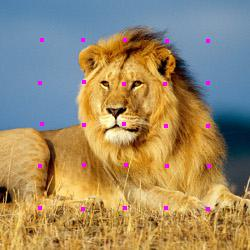
\includegraphics[height=6cm]{code/outputs/prob1a_25_centers.jpg}
  \caption{prob1a\_25\_centers}
\end{figure}
\begin{figure}[!h]
  \centering
  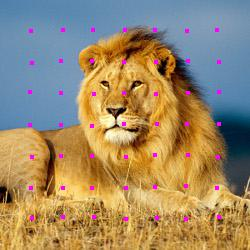
\includegraphics[height=6cm]{code/outputs/prob1a_49_centers.jpg}
  \caption{prob1a\_49\_centers}
\end{figure}
\begin{figure}[!h]
  \centering
  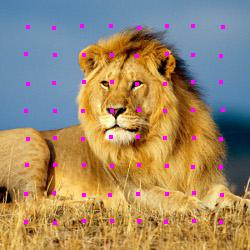
\includegraphics[height=6cm]{code/outputs/prob1a_64_centers.jpg}
  \caption{prob1a\_64\_centers}
\end{figure}
\begin{figure}[!h]
  \centering
  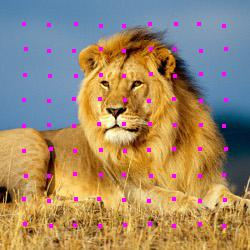
\includegraphics[height=6cm]{code/outputs/prob1a_81_centers.jpg}
  \caption{prob1a\_81\_centers}
\end{figure}
\begin{figure}[!h]
  \centering
  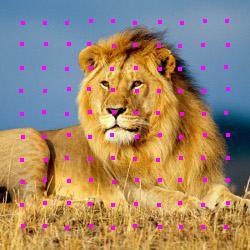
\includegraphics[height=6cm]{code/outputs/prob1a_100_centers.jpg}
  \caption{prob1a\_100\_centers}
\end{figure}

\spart{b} The results are shown as follow. Value of \textbf{spatial\_weight} is 0.3, which is chosen based on experiment result.
Larger the value is, more blocks the results have. So, the value should be a small constant. 
On the contrary, if the value is too small, we can not find a integral cluster. Points in the same scatter in many places.

\begin{figure}[!h]
  \centering
  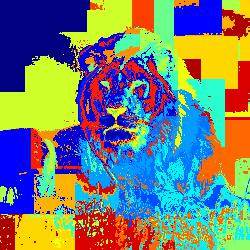
\includegraphics[height=6cm]{code/outputs/prob1b_25.jpg}
  \caption{prob1b\_25}
\end{figure}
\begin{figure}[!h]
  \centering
  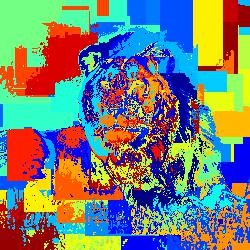
\includegraphics[height=6cm]{code/outputs/prob1b_49.jpg}
  \caption{prob1b\_49}
\end{figure}
\begin{figure}[!h]
  \centering
  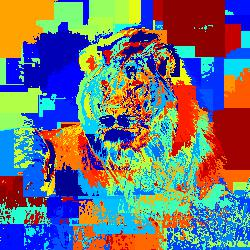
\includegraphics[height=6cm]{code/outputs/prob1b_64.jpg}
  \caption{prob1b\_64}
\end{figure}
\begin{figure}[!h]
  \centering
  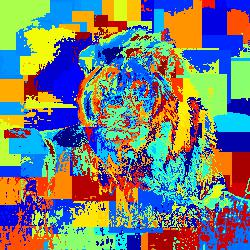
\includegraphics[height=6cm]{code/outputs/prob1b_81.jpg}
  \caption{prob1b\_81}
\end{figure}
\begin{figure}[!h]
  \centering
  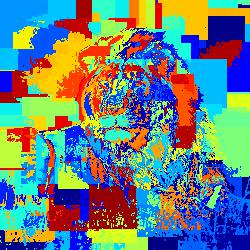
\includegraphics[height=6cm]{code/outputs/prob1b_100.jpg}
  \caption{prob1b\_100}
\end{figure}

\solution{2} 
\spart{a} 
I try different batch size, learning rate and number of hidden units and the results are shown as follow.
The limits of the uniform distribution is for the stable of training process. 
For example, if the initial value is too large compared with the gradient, then training process will take too much time.
And if the initial in different layer have huge difference, the changing of value of these parameters in training process are not in the same rate, which makes training process unstable.

\spart{b}
I did some experiment with different learning rate and batch size under condition of using momentum or using SGD. The result is shown as follow.
Basically, momentum help training process become quick and stable and have better performance in both loss value and accuracy when training or validating.

\begin{figure}[!h]
  \centering
  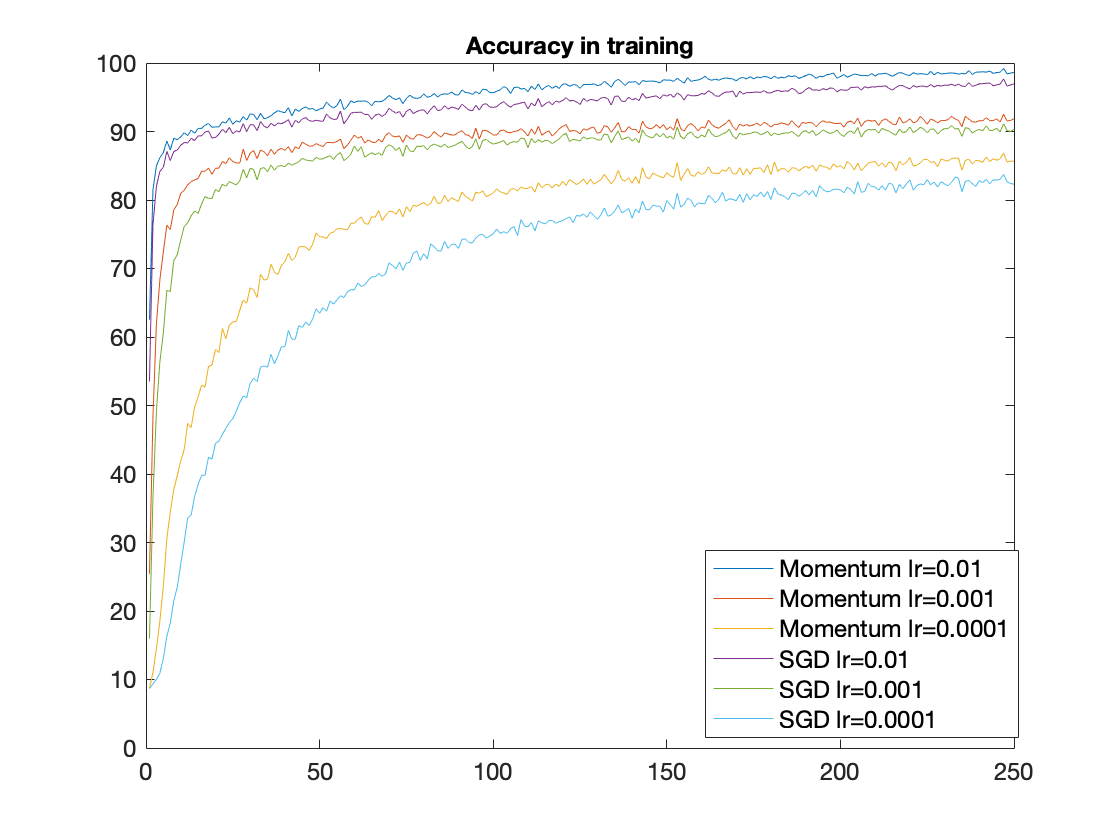
\includegraphics[height=8cm]{plots/at_lr.png}
  \caption{Accuracy in Training with Different Learning Rate}
\end{figure}
\begin{figure}[!h]
  \centering
  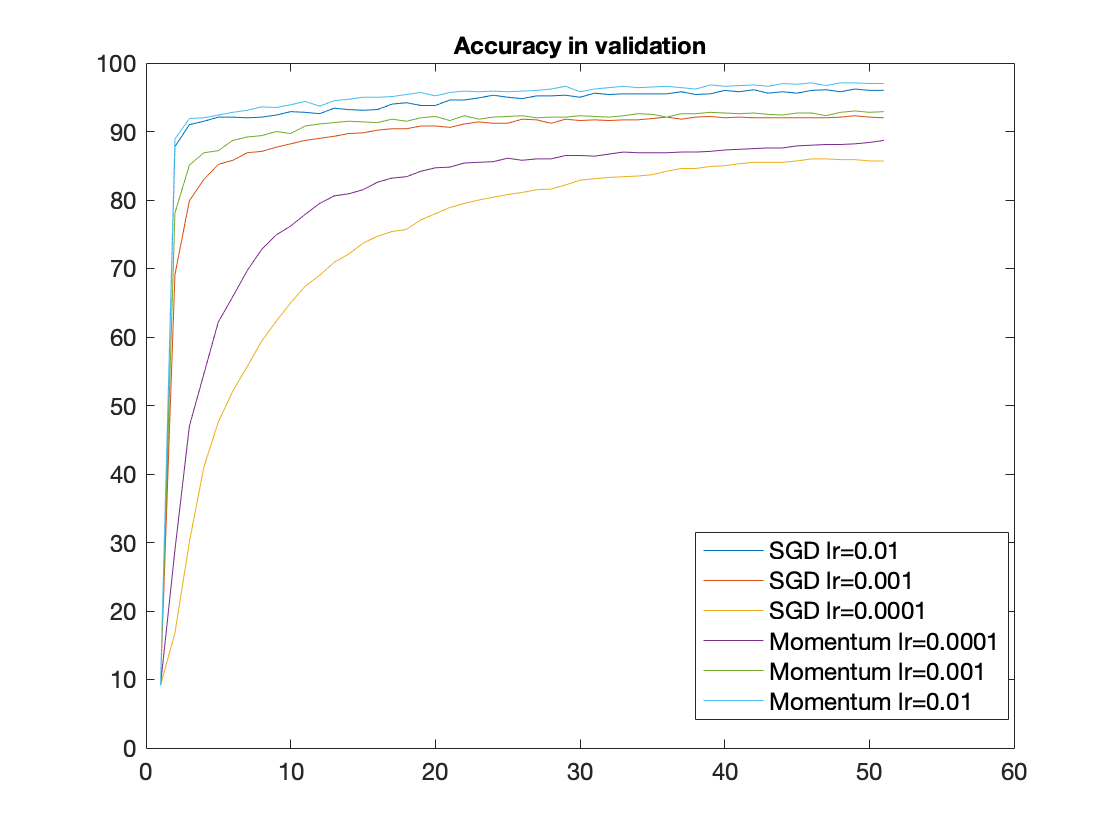
\includegraphics[height=8cm]{plots/av_lr.png}
  \caption{Accuracy in Validation with Different Learning Rate}
\end{figure} 
\begin{figure}[!h]
  \centering
  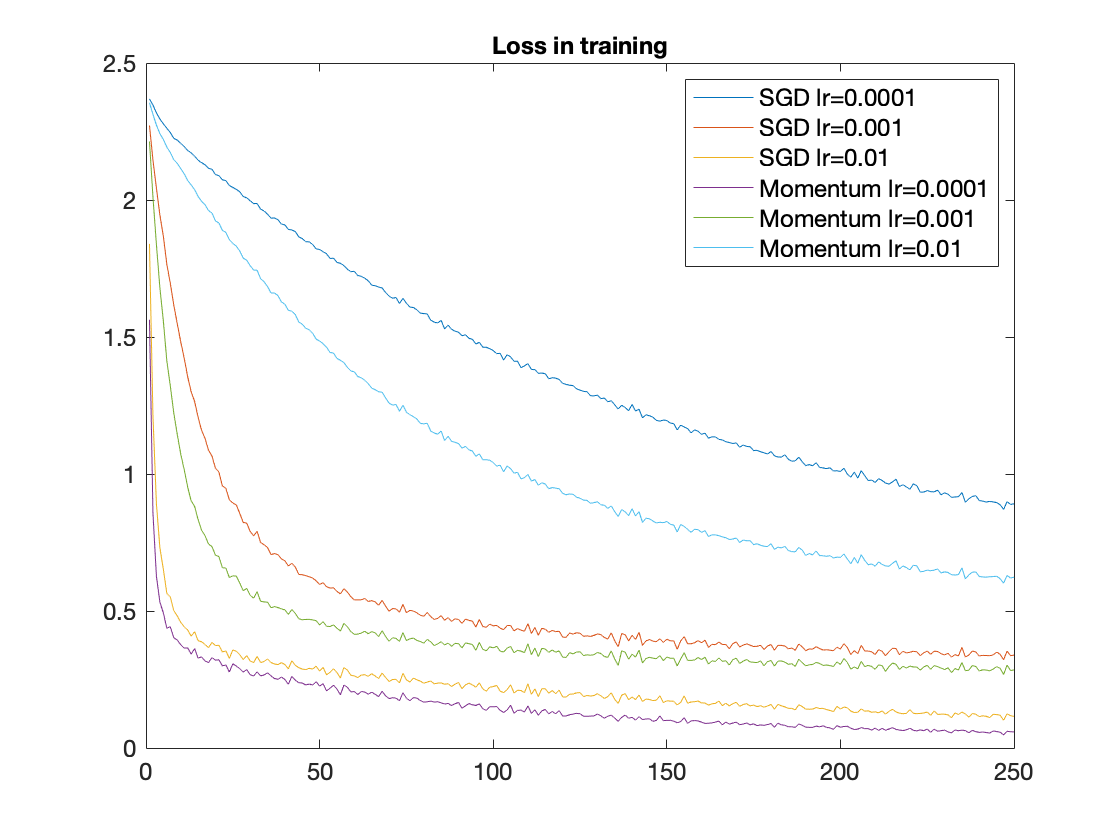
\includegraphics[height=8cm]{plots/lt_lr.png}
  \caption{Loss in Training with Different Learning Rate}
\end{figure}
\begin{figure}[!h]
  \centering
  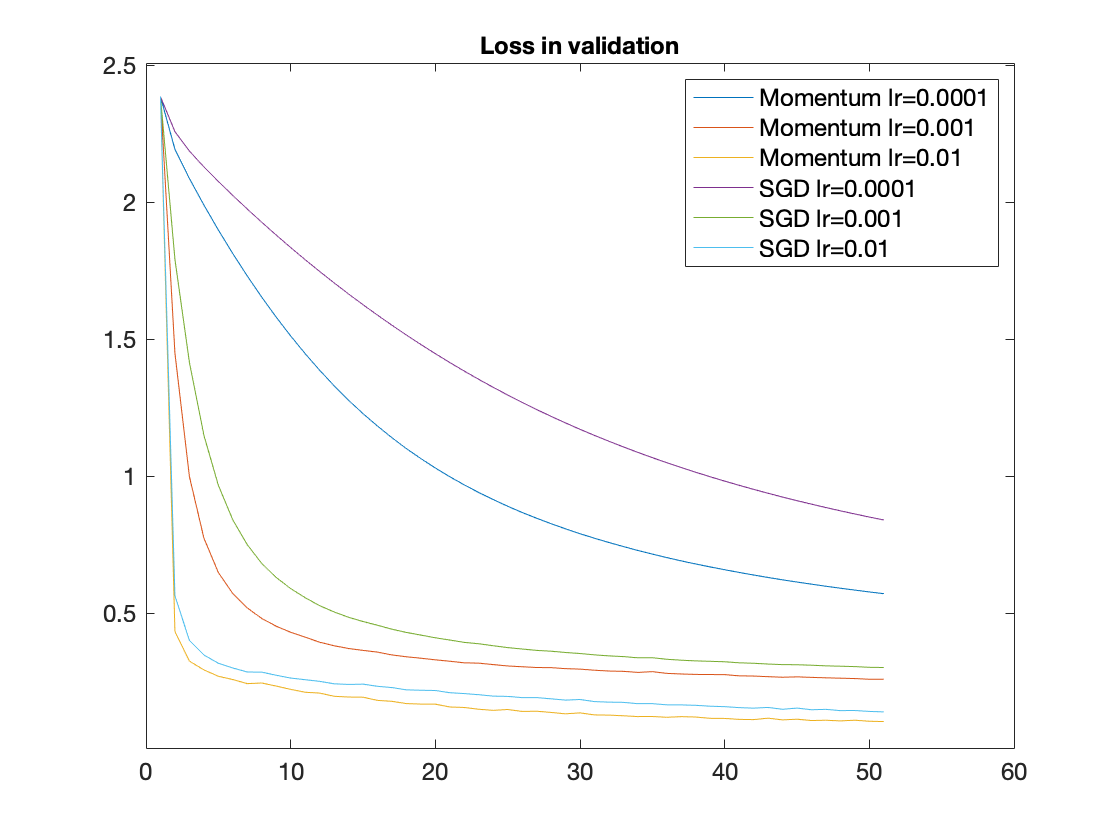
\includegraphics[height=8cm]{plots/lv_lr.png}
  \caption{Loss in Validation with Different Learning Rate}
\end{figure}
\begin{figure}[!h]
  \centering
  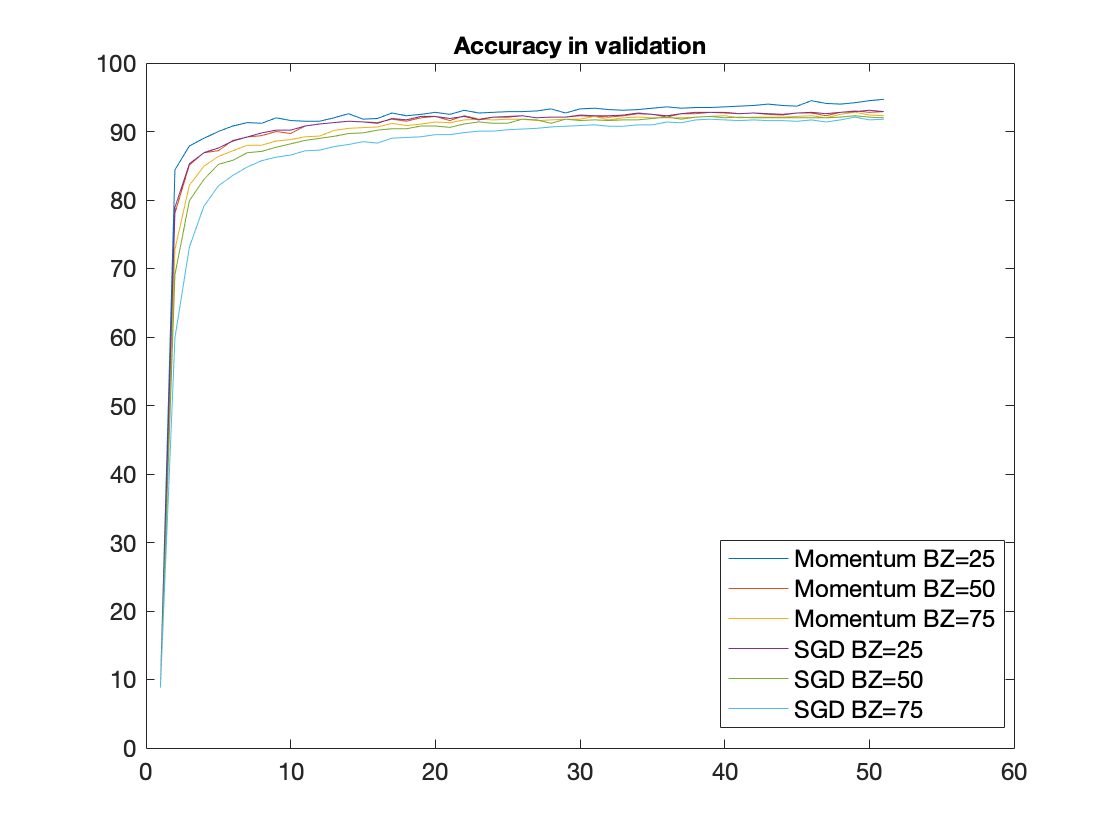
\includegraphics[height=8cm]{plots/av_bz.png}
  \caption{Accuracy in Training with Different Batch Size}
\end{figure}
\begin{figure}[!h]
  \centering
  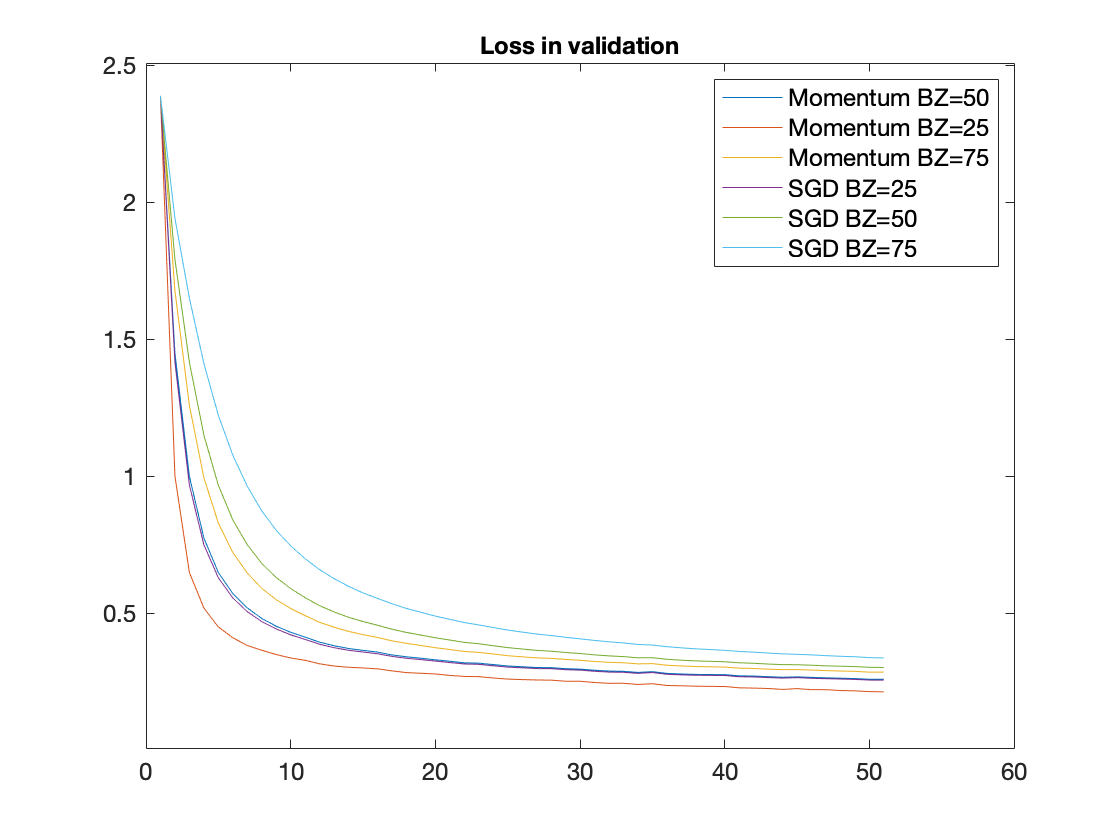
\includegraphics[height=8cm]{plots/lv_bz.png}
  \caption{Accuracy in Validation with Different Batch Size}
\end{figure}

\solution{3} 
I did some experiment with momentum and default parameters (lr=0.001, batch size=50) under condition of using convolutional layer or not. The result is shown as follow.

\begin{figure}[!h]
  \centering
  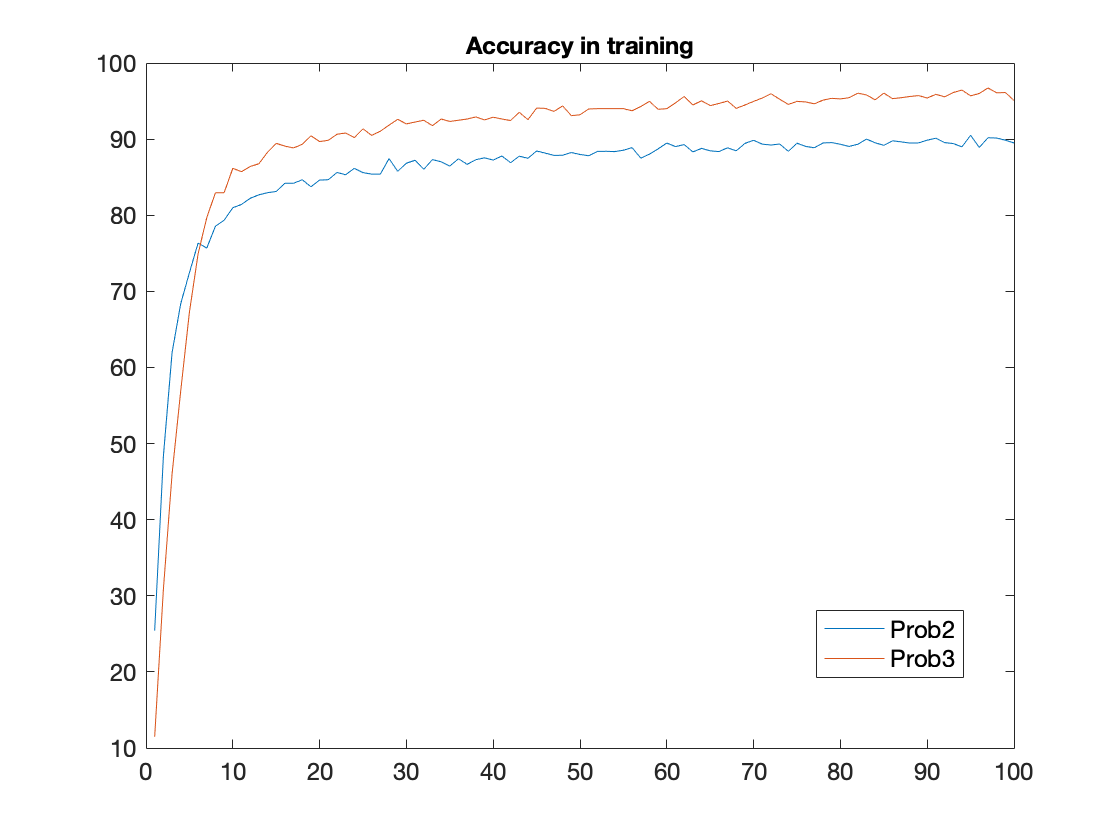
\includegraphics[height=8cm]{plots/prob3at.png}
  \caption{Accuracy in Training}
\end{figure}
\begin{figure}[!h]
  \centering
  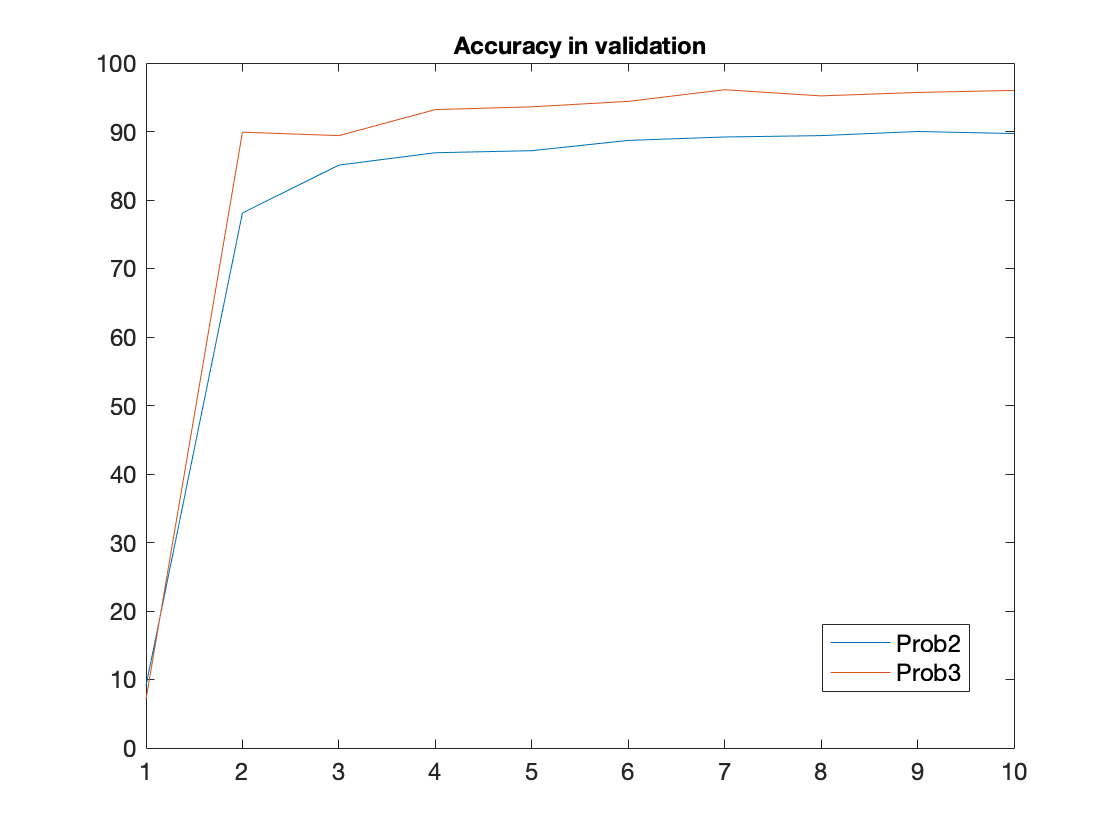
\includegraphics[height=8cm]{plots/prob3av.png}
  \caption{Accuracy in Validation}
\end{figure}
\begin{figure}[!h]
  \centering
  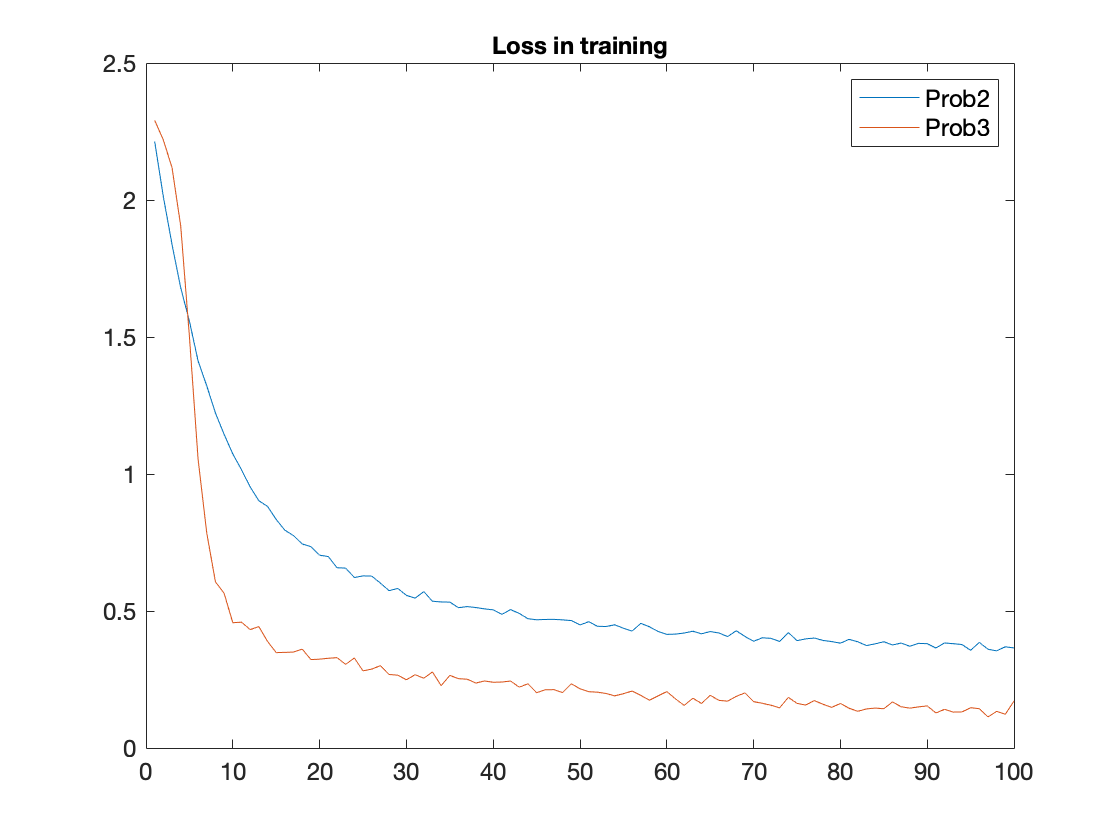
\includegraphics[height=8cm]{plots/prob3lt.png}
  \caption{Loss in Training}
\end{figure}
\begin{figure}[!h]
  \centering
  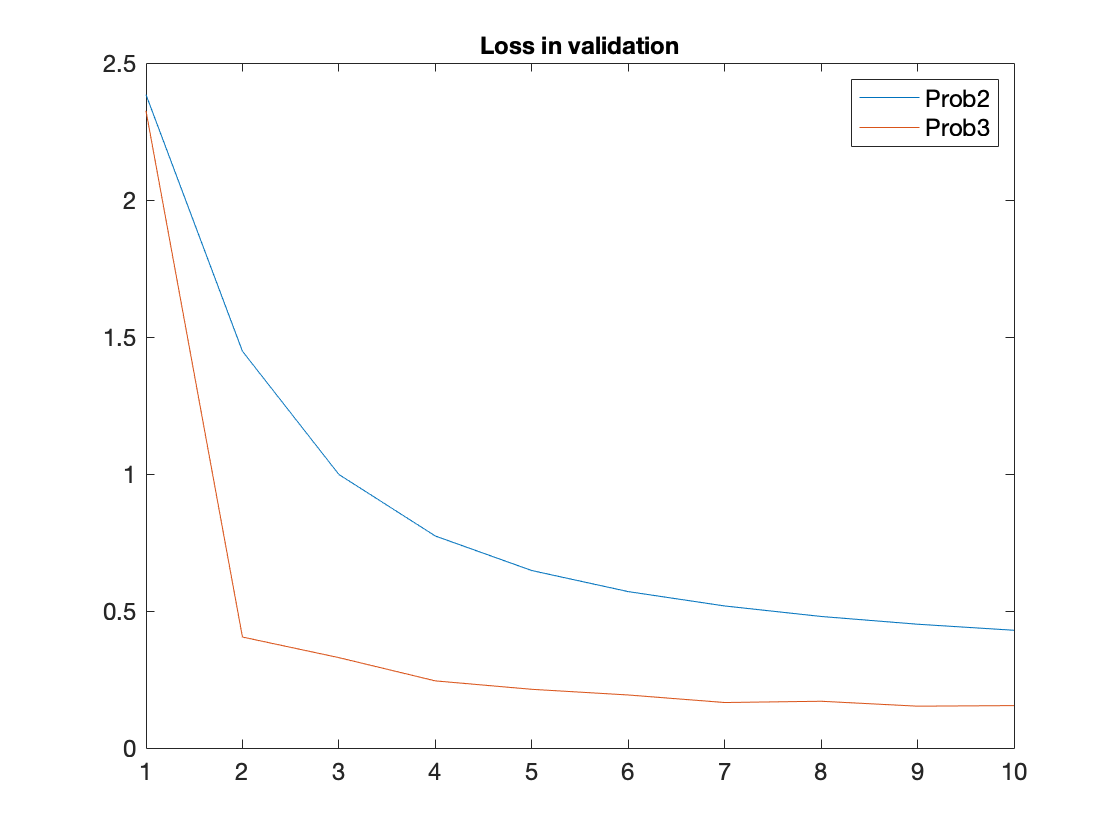
\includegraphics[height=8cm]{plots/prob3lv.png}
  \caption{Loss in Validation}
\end{figure}

%%%%%%%%%% Important, you must edit and complete the informational
%%%%%%%%%% section below. If you discussed the problem set with no
%%%%%%%%%% one, edit it to say no discussions or external resources.
\info

This problem set took approximately 18 hours of effort.

% I discussed this problem set with:
% \begin{itemize}
% \item A
% \item B
% \item C
% \end{itemize}

% Note that you might have to escape some special symbols in URLS like \_
% I also got hints from the following sources:
% \begin{itemize}
% \item Wikipedia article on matrix calculus at https://en.wikipedia.org/wiki/Matrix\_calculus
% \item Read numpy tutorial from https://docs.scipy.org/doc/numpy-1.13.0/user/basics.broadcasting.html
% \end{itemize}

\end{document}
